\subsection{\textbf{\uppercase{Desenvolvimento da Suíte de Testes Automatizados}}}

A suíte de testes automatizados possui a responsabilidade de garantir o correto funcionamento da integração entre os sistemas envolvidos, ou seja prover um meio onde possa ser testado o Webservice do GSAN e o Middleware juntamente com o Asterisk. 
Neste cenário foram utilizados recursos do JUnit e Asterisk-Java. O \textit{framework} JUnit \ref{key:annotation} foi utilizado para criação dos cenários de teste, execução dos testes e identificação de falhas. Para estabelecer uma conexão com o Asterisk, criar e monitorar chamadas telefônicas com parametrização dinâmica foram utilizados recursos do \textit{framework} Asterisk-Java \ref{key:asteriskjava}.  

A execução dos testes através do \textit{framework} JUnit podem ser realizada a qualquer momento, seja manualmente pela IDE de desenvolvimento ou automatizada por algum ambiente de Integração Contínua\footnote{Integração Contínua adotada na Engenharia de Software refere-se a uma prática de unir todo o trabalho desenvolvido várias vezes ao dia em uma estrutura principal.}. Dessa forma é possível realizar a inspeção da qualidade do software, visando garantir o correto comportamento dos sistemas na construção de uma entrega ou \textit{release}.

A suíte de teste é composta pelos seguintes classes;
\begin{itemize}
	\item Constantes - Contém a parametrização necessária para configuração da conexão com a ferramenta Asterisk.
	\item Serviço - Permite efetuar o \textit{Login}, \textit{Logoff} e iniciar uma chamada telefônica.
	\item Testes - Implementa a lógica do cenário de teste.
	\item Utilitária - Realiza o registro de ouvintes em chamadas telefônicas.
\end{itemize}


Com o intuito de unir os recursos do \textit{framework} JUnit com os do Asterisk-Java, cada classe de teste deve seguir um padrão no momento da implementação, conforme descrito a seguir:

\begin{enumerate}
	\item Configurar o método de Teste anotado com \textit{@Test}.
	\item Configurar o método de \textit{Login} anotado com \textit{@Before}.
	\item Configurar o método de \textit{Logoff} anotado com \textit{@After}.
	\item Implementar uma interface chamada \textit{PropertyChangeListener}.	
\end{enumerate}

Por meio desta padronização na classe de teste, permite que a mesma seja executada pelo \textit{framework} JUnit e se comunique com a ferramenta Asterisk por meio do \textit{framework} Asterisk-Java.

O diagrama sequência demostrado na figura \ref{figura:diagramaSeq2Via} ilustra o funcionamento da classe de teste do serviço Obter 2ª via de conta, trabalhando em conjunto com a suíte de teste.

Esse modelo é atributo a todos os testes de integração desenvolvidos na suíte de testes, onde inicialmente é realizado o processo de Login junto a ferramenta Asterisk, em seguida é criada a chamada utilizando o método \textit{sendAction}, e registrado o ouvinte através do método \textit{addListener}, quando o Asterisk identifica mudança nas propriedades da chamada do ouvinte registrado, dispara o método \textit{propertyChange} contendo os detalhes do evento, com esses detalhes o teste por determinar o ocorrência e sucesso ou error e posteriormente remove o registro de ouvinte e realiza o \textit{Logoff}, chamando respectivamente os métodos \textit{removeListener} e \textit{Logoff}.

\begin{figure}[H]
	\centering
	\caption{Diagrama de sequência utilizando a suíte de teste.}
	\label{figura:diagramaSeq2Via}
	\begin{subfigure}[H]{\textwidth}
		\centering
		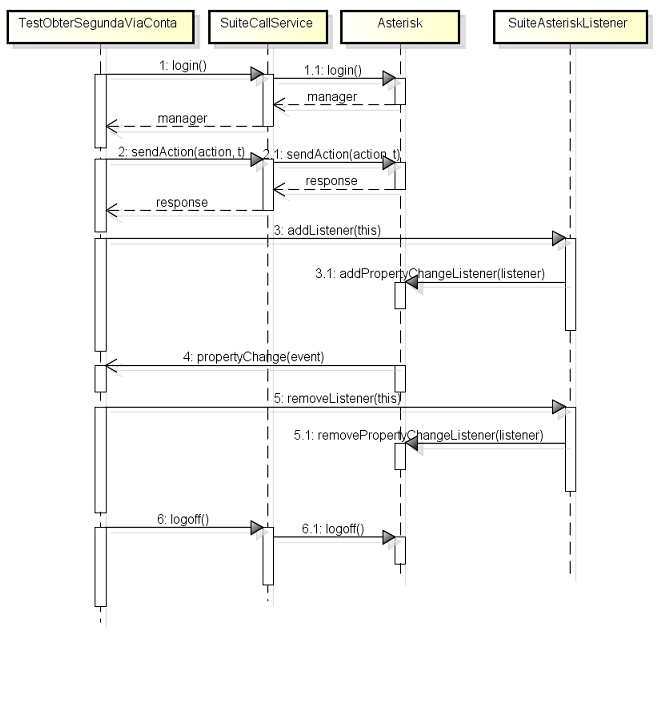
\includegraphics{figuras/diagramaSequenciaObter2Via.png}
		\legend {\fontsize{10}{12}\selectfont {Fonte: Autoria Própria}.}	
	\end{subfigure}
\end{figure}


Durante a execução de um cenário de teste, é necessário monitorar o comportamento da chamada ou canal internamente na ferramenta Asterisk,
a fim de validar o retorno obtido pela requisição e posteriormente evidenciar a ocorrência do comportamento esperado ou de falhas. Com isso se faz necessário habilitar a conexão remota na ferramenta Asterisk. O arquivo \textit{/etc/asterisk/manager.conf} contém as propriedades necessárias para serem configuradas, a seguir é demostrada a configuração realizada para execução dos testes automatizados:
\\
\hspace{10 mm}\textit{[general]} 			\hspace{10 mm} $\triangleright$ Contexto geral de conexão.\\
\hspace{10 mm}\textit{enabled=yes}  		\hspace{10 mm} $\triangleright$ Habilitar a conexão remota.\\
\hspace{10 mm}\textit{port=5038}  			\hspace{10 mm} $\triangleright$ Define a porta.\\
\hspace{10 mm}\textit{displayconnects=yes}  \hspace{10 mm} $\triangleright$ Define a exibição das conexões no console.\\
\hspace{10 mm}\textit{permit=0.0.0.0/0.0.0.0} \hspace{10 mm} $\triangleright$ Define o endereço IP que será aceito.\\

Abaixo segue o exemplo de configuração para adição de um novo usuário para conexão remota:
\\
\hspace{10 mm}\textit{[manager]} 	\hspace{10 mm} $\triangleright$ Nome do novo usuário.\\
\hspace{10 mm}\textit{secret=pa55w0rd} \hspace{10 mm} $\triangleright$ Senha do novo usuário \\
\hspace{10 mm}\textit{read=system,call,log,verbose,command,agent}  \hspace{10 mm} $\triangleright$ Define as permissões de leitura.\\
\hspace{10 mm}\textit{write=system,call,log,verbose,command,agent}  \hspace{10 mm} $\triangleright$ Define as permissões de escrita.\\
\hspace{10 mm}\textit{permit=0.0.0.0/0.0.0.0} \hspace{10 mm} $\triangleright$ Define o endereço IP que será aceito \\


A distribuição Disc-OS por padrão possui uma configuração de \textit{firewall} bastante restritiva por questões de segurança, para que não ocorra rejeição nas solicitações realizadas ao Asterisk, será para fins de testes desabilitada as regras do \textit{firewall}, utilizando o seguinte comando \textit{/etc/init.d/iptables stop}.
 
A suíte de testes contém a implementação dos testes de integração para os três serviços automatizados que são obter 2º via de conta, informar falta de água e solicitar restabelecimento da ligação de água, além de testes unitários para verificação da rotina de enviar e-mail e checagem da disponibilidade do \textit{Webservice}.
A vantagem principal obtida por meio da suíte de testes se trata da possibilidade de tornar o processo de identificação de falhas padronizado, já sua desvantagem se trata da complexidade na etapa de configuração.


